\documentclass[../DS10.tex]{subfiles}%
\graphicspath{{./figures/}}%

% \subimport{/home/nora/Documents/Enseignement/Prepa/bpep/exercices/DS/titrage_CO2/}{sujet.tex}%

\begin{document}%
\section[42]"E"{Les phénomènes d'induction -- QCM}

\enonce{%
	Indiquer la ou les bonnes propositions pour chaque question et
  \textbf{justifiez entièrement} vos choix.
}%

\QR[4]{%
  Soit $\vv{B}$ un champ magnétique uniforme. Que vaut le flux $\Phi$ du champ
  magnétique à travers la surface $\vv{S}$~?
	\begin{center}
		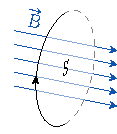
\includegraphics[width=.2\linewidth]{flux_simple}
	\end{center}
	\begin{tasks}[label=\protect\fbox{\Alph*}, label-width=4ex](4)
		\task $\F = BS$
		\task $\F = -BS$
		\task $\F = \vv{B} \cdot \vv{S}$
		\task $\F = - \vv{B} \cdot \vv{S}$
	\end{tasks}
}{%
  \fatbox{\textbf{C}}~: pour un champ magnétique uniforme, le flux de $\vv{B}$
  est, par définition~: $\Phi \stm{=} \iint_{S} \vv{B} \cdot \vv{\dd{S}} = \vv{B}
  \cdot \vv{S}$. \pt{1}
  \smallbreak
  \fatbox{\textbf{B}}~: le vecteur $\vv{S}$ étant dans le sens opposé à $\vv{B}$
  (en utilisant la règle de la main droite \pt{1} par rapport au contour
  orienté), on a $\Phi = -BS$ \pt{1}.
}%

\QR[6]{%
	Qu'est-ce qui peut faire varier le flux d'un champ magnétique extérieur à
	travers un circuit~? Donner un exemple pour chaque bonne réponse. Expliquer
  pourquoi la ou les mauvaises réponses le sont.
	\begin{tasks}[label=\protect\fbox{\Alph*}, label-width=4ex](2)
		\task un déplacement du circuit
		\task une déformation du circuit
		\task une variation du champ magnétique
		\task une variation de courant dans le circuit
	\end{tasks}
}{%
  \fatbox{\textbf{A}}~: si $\Bf$ n'est pas uniforme dans tout l'espace, le flux
  change \pt{1}.
  \smallbreak
  \xul{Exemple}~: un aimant qu'on approche d'une spire \pt{1}.
  \smallbreak
  \fatbox{\textbf{B}}~: si la surface change, le flux change \pt{1}.
  \smallbreak
  \xul{Exemple}~: les rails de \textsc{Laplace}, le mouvement du barreau change
  la surface du circuit \pt{1}.
  \smallbreak
  \fatbox{\textbf{C}}~: idem que la A \pt{1}.
  \smallbreak
  Une variation du courant dans le circuit fait varier le champ magnétique
  \textbf{propre} mais pas le champ magnétique \textbf{extérieur} \pt{1}.
}%

\QR[2]{%
	Dans la relation de Faraday $e = -\dv{\Phi}{t}$, que représente $e$ ? Répondre
  sans justification.
	\begin{tasks}[label=\protect\fbox{\Alph*}, label-width=4ex](2)
		\task une énergie
		\task une tension
	\end{tasks}
	Que représente $\Phi$~? Répondre sans justification.
	\begin{tasks}[label=\protect\fbox{\Alph*}, label-width=4ex, start=3](2)
		\task le flux d'un champ magnétique
		\task un déplacement
	\end{tasks}
}{%
  \fatbox{\textbf{B}}~: $e$ est une tension, une force électro-motrice. \pt{1}
  \smallbreak
  \fatbox{\textbf{C}}~: $\Phi$ est le flux d'un champ magnétique. \pt{1}
}%

\QR[5]{%
  On approche l'aimant de la spire en le translatant vers la droite, il en
  résulte un courant $i$.
	\begin{center}
		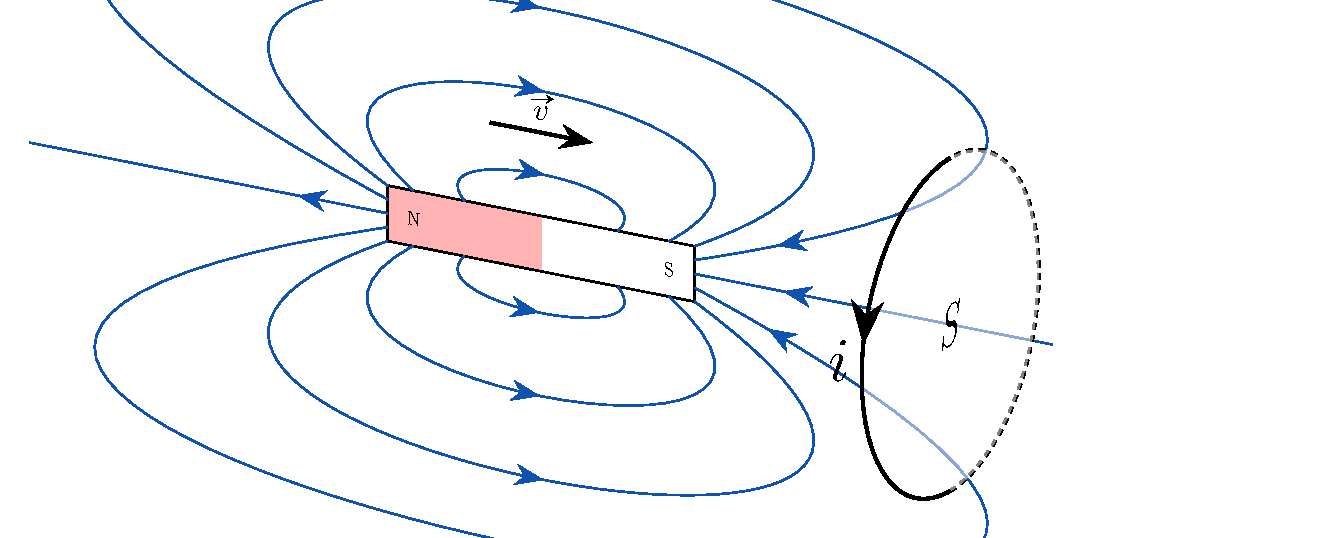
\includegraphics[width=.5\linewidth]{induc_spire}
	\end{center}
  Que peut-on dire de $i$~? Justifier entièrement. Un schéma est attendu.
	\begin{tasks}[label=\protect\fbox{\Alph*}, label-width=4ex](3)
		\task $i$ est positif.
		\task $i$ est négatif.
		\task $i$ est nul.
	\end{tasks}
}{%
	\fatbox{\textbf{A}}~:
	le champ magnétique est orienté vers la \textbf{gauche}, et son intensité
	augmente puisqu'on rapproche l'aimant. On a donc $\dv{\Bf\ind{ext}}{t}$
	\textbf{positif vers la gauche}. \pt{1}
	\smallbreak
  Comme le flux varie, il y a un phénomène d'induction \pt{1} dans la spire
  donnant lieu à une f.é.m. induite $e\ind{ind}$, elle-même donnant lieu à une
  intensité induite $i\ind{ind}$, à l'origine d'un champ propre induit
  $\Bf\ind{p,ind}$. Cette conséquence doit modérer la cause \pt{1} qui lui a
  donné naissance, donc $\dv{\Bf\ind{p,ind}}{t}$ doit être \textbf{vers la
  droite}. \pt{1}
	\smallbreak
	Avec la règle de la main droite, on sait que l'intensité qui génère ce champ
	doit être \textbf{positive} \pt{1} avec la convention tracée sur le schéma.
}%

\QR[2]{%
	Deux circuits sont en couplage mutuel. Que peut-on dire sur $u$~?
	\begin{center}
		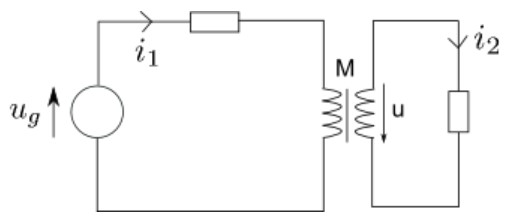
\includegraphics[width=.45\linewidth]{induction3}
	\end{center}
	\begin{tasks}[label=\protect\fbox{\Alph*}, label-width=4ex](4)
		\task $\DS u = L_1 \dv{i_1}{t} + L_2 \dv{i_2}{t}$
		\task $\DS u = M \dv{i_1}{t} + M \dv{i_2}{t}$
		\task $\DS u = L_1 \dv{i_1}{t} + M \dv{i_2}{t}$
		\task $\DS u = L_2 \dv{i_2}{t} + M \dv{i_1}{t}$
	\end{tasks}
}{%
  \fatbox{\textbf{D}}~:
  $u$ est la somme d'un terme d'inductance propre \pt{1}
  associée à $i_2$ et d'inductance mutuelle associée \pt{1} à $i_1$ circulant
  dans le circuit de gauche.
}%

\QR[4]{%
  De quoi l'inductance mutuelle $M$ dépend-elle~? Justifier chaque bonne
  \textbf{et} mauvaise réponse.
	\begin{tasks}[label=\protect\fbox{\Alph*}, label-width=4ex](2)
		\task la forme des deux circuits
		\task la position relative des deux circuits
		\task l'orientation des deux circuits
		\task des courants circulant dans les deux circuits
	\end{tasks}
}{%
  \fatbox{\textbf{A}}~:
  selon la longueur des bobines, le flux varie même à courant constant. \pt{1}
  \smallbreak
  \fatbox{\textbf{B}}~:
  idem, si on éloigne les bobines le flux varie alors que
  $i$ contant. \pt{1}
  \smallbreak
  \fatbox{\textbf{C}}~: 
  si on retourne la bobine, l'effet d'induction est opposé (règle de la main
  droite). \pt{1}
  \smallbreak
  $M$ ne dépend pas du courant circulant, puisqu'il est par définition le
  coefficient de proportionnalité entre le flux mutuel et le courant croisé.
  \pt{1}
}%

\QR[5]{%
  L'inductance propre d'un solénoïde long ($\ell\gg r$) peut être estimée par
  quelle formule (avec $\ell$ la longueur du solénoïde, $r$ son rayon, $S$ sa
  section et $N$ son nombre de spires)~? Justifier entièrement. Un schéma est
  attendu.
	\begin{tasks}[label=\protect\fbox{\Alph*}, label-width=4ex](4)
		\task $L = \frac{\mu_0 NS}{\ell}$
		\task $L = \frac{\mu_0 N\ell}{S}$
		\task $L = \frac{\mu_0 N^2S}{\ell}$
		\task $L = \frac{\mu_0 N^2\ell}{S}$
	\end{tasks}
}{%
  \fatbox{\textbf{C}}~:
  \smallbreak
  \noindent
  \begin{minipage}[c]{.4\linewidth}
    \begin{center}
        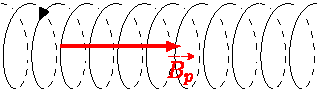
\includegraphics[scale=1]{bobib}
        \label{fig:bobi}
    \end{center}
  \end{minipage}
  \hfill
  \begin{minipage}[c]{.69\linewidth}
      $i$ et $\vv{B_p}$ respectent la règle de la main droite. \pt{1}
  \end{minipage}
    Pour $N$ spires~:
    \[
      \F_p \stm{=} N\times \vv{B_p}\cdot \vv{S}
    \]
    Or, $\vv{B_p}$ et $\vv{S}$ sont tous deux orientés à partir de $i$
    selon la règle de la main droite, donc
    \begin{gather*}
      \vv{S} = S\uz
      \qqet
      \vv{B_p} \stm{=} \mu_0 \frac{N}{\ell }i(t)\,\uz
      \qquad 
      \Lra
      \qquad 
      \boxed{\F_p = \mu_0 \frac{N^2}{\ell }Si(t)}
    \end{gather*}
    Or,
    \[
      \F \stm[-1]{=} Li
      \Lra
      \boxed{L \stm[-1]{=} \mu_0 \frac{N^2}{\ell }S}
    \]
}%

\QR[2]{%
	Une bobine fermée sur elle même est soumise à un champ magnétique extérieur
	$\vv{B\ind{ext}}$ variable, et à son champ propre $\vv{B\ind{p}}$. On la
	représente par le circuit équivalent, où $R$ représente sa résistance interne.
	\begin{center}
		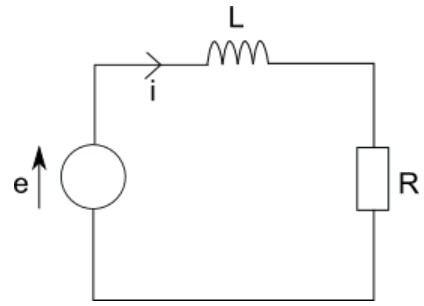
\includegraphics[width=.3\linewidth]{induction4}
	\end{center}
	$e$ modélise l'effet de
	\begin{tasks}[label=\protect\fbox{\Alph*}, label-width=4ex](2)
		\task $\Bf\ind{ext}$
		\task $\Bf\ind{p}$
	\end{tasks}
	$L$ modélise l'effet de
	\begin{tasks}[label=\protect\fbox{\Alph*}, label-width=4ex, start=3](2)
		\task $\Bf\ind{ext}$
		\task $\Bf\ind{p}$
	\end{tasks}
}{%
  \fatbox{\textbf{A}}~:
	$e$ modélise l'effet d'induction associé à la variation du flux du champ
	magnétique extérieur. \pt{1}
  \smallbreak
  \fatbox{\textbf{D}}~:
  la bobine d'inductance $L$ modélise l'effet
	auto-inductif, c'est-à-dire la variation du flux du champ magnétique propre.
  \pt{1}
}%

\QR[7]{%
	Un barreau est posé immobile sur les rails de Laplace et un générateur de fem
	$E>0$ est allumé à l'instant initial. On ne \textbf{néglige pas l'induction}.
  Quel(s) scénario(s) suivant(s) est (sont) vrai(s)~? Expliquer.
	\begin{center}
		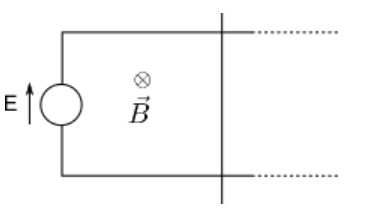
\includegraphics[width=.3\linewidth]{induction5}
	\end{center}
	\begin{tasks}[label=\protect\fbox{\Alph*}, label-width=4ex](2)
		\task Le barreau reste immobile.
		\task Le barreau est mis en mouvement vers la gauche.
		\task Le barreau est mis en mouvement vers la droite.
		\task Le barreau atteint une vitesse limite.
	\end{tasks}
}{%
  \fatbox{\textbf{C}}~:
  le circuit est conducteur. La force électro-motrice extérieure $E$ va donc
  mettre en mouvement les électrons et un courant circulant du haut vers le bas
  va circuler dans le barreau \pt{1}.
  \smallbreak
  La force de \textsc{Laplace} $\Ff\ind{lap} = i
  \vv{L} \wedge \Bf$ \pt{1} est alors orientée vers la \textbf{droite}, qui est
  donc le sens du barreau \pt{1}.
	\smallbreak
  \fatbox{\textbf{D}}~:
  le mouvement du barreau induit lors une variation du flux du champ magnétique
  \pt{1}, induisant à son tour une force électro-motrice $e$ s'opposant à $E$
  (par loi de \textsc{Lenz}) \pt{1}.
  \smallbreak
  Plus le barreau accélère et plus $e$
  augmente, jusqu'à compenser $E$. \pt{1} Le courant devient alors nul, la force
  de \textsc{Laplace} également et le barreau atteint une vitesse limite \pt{1}.
}%

\QR[2]{%
	Un barreau de taille $\SI{10}{cm}$ est posé sur des rails de Laplace. On
	mesure un champ magnétique de $\SI{100}{mT}$ et un courant de $\SI{1}{A}$.
	Combien vaut la norme de la force de Laplace subie par le barreau ?
	\begin{tasks}[label=\protect\fbox{\Alph*}, label-width=4ex](4)
		\task \SI{10}{N}
		\task \SI{1}{N}
		\task \SI{0.1}{N}
		\task \SI{0.01}{N}
	\end{tasks}
}{%
  \fatbox{\textbf{D}}~:
	la norme de la force de Laplace est égale au produit $i\ell B$ \pt{1}. Ainsi,
	\[
		F\ind{L} = \SI{0,01}{N}
    \qquad 
    \pt{1}
	\]
}%

\QR[4]{%
	On considère un pendule pesant oscillant dont l'extrémité est une lame
	métallique conductrice. On approche alors un aimant. Que se passe-t-il~?
  Expliquer.
	\begin{center}
		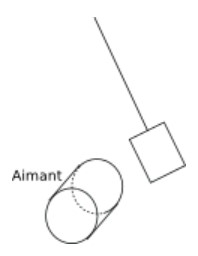
\includegraphics[width=.25\linewidth]{induction6}
	\end{center}

	\begin{tasks}[label=\protect\fbox{\Alph*}, label-width=4ex](2)
		\task L'aimant entretient les oscillations.
		\task L'aimant amortit les oscillations.
		\task La lame de métal s'échauffe.
		\task La lame de métal refroidit.
	\end{tasks}
}{%
  \fatbox{\textbf{B}}~:
  par loi de \textsc{Lenz} \pt{1}, les effets inductifs vont s'opposer aux
  causes. La cause étant ici le mouvement relatif du pendule par rapport à
  l'aimant, on s'attend à ce que les effets inductifs (donc l'aimant) amortisse
  les oscillations \pt{1}.
  \smallbreak
  \fatbox{\textbf{C}}~: des courants de \textsc{Foucault} \pt{1} sont induits
  dans la lame de métal qui s'échauffe alors par effet \textsc{Joule} \pt{1}.
}%
\end{document}
